\documentclass[11pt]{beamer}
%\usepackage{nopageno}
%\usepackage{textgreek}
\usepackage{silence}
\usepackage{appendix}
\WarningsOff[tikz-feynman]
\usepackage{float}
%\usepackage[utf8]{inputenc}
\usepackage[english]{babel}
\usepackage{caption}
\usepackage{subcaption}
\usepackage{amsmath}
\numberwithin{equation}{section}
\DeclareMathOperator{\Tr}{Tr}
\usepackage{amsfonts}
\usepackage{amssymb}
\usepackage{slashed}
\usepackage{graphicx}
\usepackage{datetime}
\usepackage[compat=1.1.0]{tikz-feynman}

\usetheme{metropolis}
\usepackage[utf8]{inputenc}
\usepackage[english]{babel}
\usepackage{amsmath}
\usepackage{amsfonts}
\usepackage{amssymb}
\usepackage{graphicx}
\author{Gerrit Bickendorf}
\title{Leptophilic Dark Matter}
\setbeamercovered{transparent} 
%\setbeamertemplate{navigation symbols}{} 
%\logo{} 
%\institute{} 
\date{April 23, 2019} 
%\subject{} 
\begin{document}
\beamertemplatenavigationsymbolsempty
\begin{frame}
\titlepage
\end{frame}

%\begin{frame}
%\tableofcontents
%\end{frame}

\begin{frame}{Outline}
\begin{itemize}
\pause
\item Introduce need for leptophilic mediators
\pause
\item Introduce a vector and scalar model
\pause
\item Constrains from muon decay spectrum
\pause
\item Constrains from lepton universality in $\pi^+$ decays
\pause
\item Constrains from $\pi^+$ decay spectrum
\end{itemize}
\end{frame}

\begin{frame}{Introduction}
\begin{itemize}
\item Need dark matter to stay dark \\
\pause
$\rightarrow$ Introduce secluded dark sector without SM interactions
\pause 
\item Only interaction: Through mediator
\pause
\item Try to constrain mediator models
\end{itemize}
\end{frame}

\begin{frame}{Leptophilic Mediator}
\begin{itemize}
\item Why is there only indirect evidence for states beyond the standard model?
\pause
\item No tree level coupling to quarks and SM-gauge bosons
\pause
\item Only direct coupling to leptons\\
$\rightarrow$ "Leptophilic"
\end{itemize}
\end{frame}

\begin{frame}{Vector Model}
\begin{align*}
\mathcal{L}=& \mathcal{L}_\text{SM}-\frac{1}{4}F_{\mu\nu}'F'^{\mu\nu}+\frac{m_{A'}^2}{2}A_\mu'A'^\mu +\frac{\epsilon}{2}F_{\mu\nu}'F^{\mu\nu}\\
&-\sum_{l=e,\mu,\tau} e'_l\left(\bar{l}\gamma^\mu A'_\mu l+\bar{\nu}_l\gamma^\mu A'_\mu \nu_l\right)\\&+\bar{\chi}(i\slashed{\partial}-m_\chi)\chi -g_D\bar{\chi}\gamma^\mu A_\mu'\chi
\end{align*}
\end{frame}

\begin{frame}{Vector Model}
\begin{figure}[H]
\centering
\begin{tikzpicture}
\begin{feynman}[layered layout]
\vertex (in){\(\gamma\)};
\vertex [right=of in](a);
\vertex [right=of a](b);
\vertex [right=of b](out){\(A'\)};
\diagram* {
(in)--[boson](a) -- [fermion,half left,edge label=\(f\)] (b) -- [fermion,half left] (a),
(b)--[boson](out)};
\end{feynman}
\end{tikzpicture}
\end{figure}
\pause
\begin{equation*}
\epsilon =\sum_l \frac{ee_l'}{12\pi^2}\ln\left(\frac{m_\tau^2}{\mu^2}\right)
\label{eq:KinMix}
\end{equation*}
\pause
After diagonalisation:
\begin{equation*}
\mathcal{L}\supset e\epsilon A'_\mu J_{em}^\mu
\end{equation*}
\end{frame}

\begin{frame}{Scalar Model}
\begin{align*}
\mathcal{L}=& \mathcal{L}_\text{SM}+\frac{1}{2}\partial_\mu \phi \partial^\mu \phi-\frac{m_{\phi}^2}{2}\phi -\sum_{l=e,\mu,\tau} e'_l\bar{l} l \phi \\&+\bar{\chi}(i\slashed{\partial}-m_\chi)\chi -g_D\bar{\chi}\chi\phi
\end{align*}
\begin{itemize}
\pause
\item From effective dim. 5 operator 
\begin{equation*}
\frac{c_l}{\Lambda}\phi \bar{L}_i\Phi e_{iR}+h.c.
\end{equation*} 
\pause
\item After SSB
\begin{equation*}
e'_l=\frac{c_l v}{\Lambda\sqrt{2}}.
\end{equation*}
\end{itemize}
\end{frame}

\begin{frame}{Experimental constrains}
Neutrino Trident Production
\pause
\begin{figure}[H]
\centering
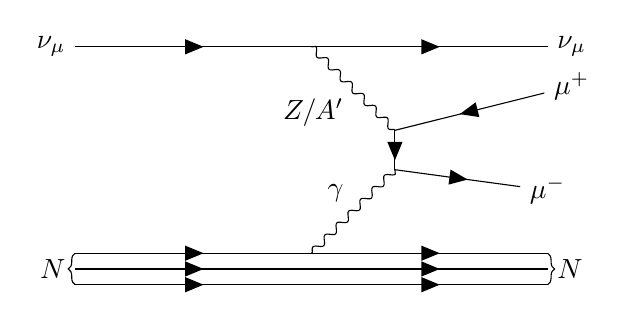
\begin{tikzpicture}
\begin{feynman}
\vertex (a1);
\vertex [above=0.2cm of a1](a2);
\vertex [above=0.2cm of a2](a3);
\vertex [right=3cm of a1](b1);
\vertex [right=3cm of a2](b2);
\vertex [right=3cm of a3](b3);
\vertex [right=3cm of b1](c1);
\vertex [right=3cm of b2](c2);
\vertex [right=3cm of b3](c3);
\vertex [above right=1.5cm of b3](d);

\vertex [above=0.5cm of d](e);


\vertex [above left=1.5cm of e](h1);
\vertex [left=3cm of h1](g1){\(\nu_\mu\)};
\vertex [right=3cm of h1](g2){\(\nu_\mu\)};
\vertex [above=0.5cm of c3](f1){\(\mu^-\)};
\vertex [below=0.5cm of g2](f2){\(\mu^+\)};;
\diagram* {
(a1) -- [fermion](b1) -- [fermion](c1),
(a2) -- [fermion](b2) -- [fermion](c2),
(a3) -- [fermion](b3) -- [fermion](c3),
(b3) -- [boson,edge label=\(\gamma\)](d),
(f2) --[fermion](e) -- [fermion](d) -- [fermion](f1),
(g1) -- [fermion](h1) -- [fermion](g2),
(e) -- [boson,edge label=\(Z/A'\)](h1)
};
\draw [decoration={brace}, decorate] (a1.south west) -- (a3.north west)
node [pos=0.5, left] {\(N\)};
\draw [decoration={brace}, decorate] (c3.south west) -- (c1.north west)
node [pos=0.5, right] {\(N\)};
\end{feynman}
\end{tikzpicture}
\end{figure}
\pause
Contribution to  \cite{Altmannshofer:2014pba}
\begin{equation*}
\frac{\sigma_{CCFR}}{\sigma_{SM}}=0.82\pm 0.28
\end{equation*}
\end{frame}

\begin{frame}{Experimental constrains}
NA64 \cite{Banerjee:2018vgk}:
\begin{itemize}
\item Missing energy search for invisible dark photo decay
\begin{equation*}
e^-N \rightarrow e^-N A' (A' \rightarrow \bar{\chi}\chi)
\end{equation*}
\item Only $m_{A'}>1MeV$
\end{itemize}
\begin{figure}[H]
\centering
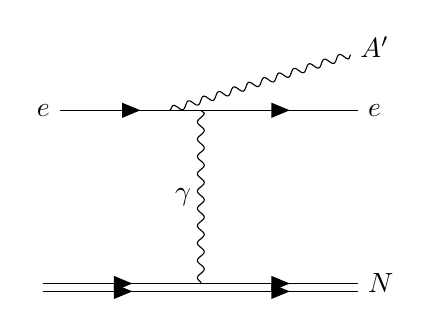
\begin{tikzpicture}
\begin{feynman}
\vertex (a1);
\vertex [above=0.1cm of a1](a2);
\vertex [right=2cm of a1](b1);
\vertex [right=2cm of a2](b2);
\vertex [right=2cm of b1](c1);
\vertex [right=2cm of b2](c2){\(N\)};
\vertex [above=2cm of a2](a3){\(e\)};
\vertex [right=2cm of a3](b3);
\vertex [right=1.6cm of a3](c);
\vertex [right=2cm of b3](c3){\(e\)};
\vertex	[above=0.8cm of c3](f1){\(A'\)};


\diagram* {
(a1) -- [fermion](b1)--[fermion](c1),
(a2) -- [fermion](b2)--[fermion](c2),
(a3) -- [fermion](b3)--[fermion](c3),
(b2) --[boson,edge label=\(\gamma\)](b3),
(c) -- [boson](f1)
};
\end{feynman}
\end{tikzpicture}
\end{figure}
\end{frame}

\begin{frame}{Experimental constrains}
BABAR:
\begin{itemize}
\item $e^+e^-$ collider process:
\begin{equation*}
e^+e^-\rightarrow \gamma A' (A' \rightarrow \bar{\chi}\chi)
\end{equation*}
\pause
\item Detect mono photon events with CM energy $E_\gamma^*$ and search for peak in $M_X^2=s-2E_\gamma^* \sqrt{s}$ 
\pause
\item $0 < m_{A'} < 8GeV$
\end{itemize}
\end{frame}

\begin{frame}{Experimental constrains}
Atomic physics \cite{Delaunay:2017dku} :
\begin{itemize}
\item Additional scalars add potential:
\begin{equation*}
V^{ij}(r)=-\frac{e_i'e_j'}{4\pi}\frac{e^{-m_\phi}}{r}
\end{equation*}
\pause
$\rightarrow$ Energy shift
\pause
\item Positronium ($e^+e^-$) 1S-2S transition\\
\pause
$\rightarrow$ bound on $e_e'$
\pause
\item Muonium ($e^-\mu^+$) 1S-2S transition and Lamb shift \\
\pause
$\rightarrow$ bound on $e_e'\times e_\mu'$
\end{itemize}

\end{frame}

\begin{frame}{Standard Model Muon Decay}
\begin{figure}[H]
\centering
\begin{tikzpicture}
\begin{feynman}
\vertex (a) {\(\mu^{-}\)};
\vertex [right=of a] (b);
\vertex [above right=of b] (f1){\(\nu_\mu \)};
\vertex [below right=of b] (c);
\vertex [above right=of c] (f2){\(e^-\)};
\vertex [below right=of c] (f3){\(\bar{\nu}_e\)};
\diagram* {
(a)--[fermion](b)--[fermion](f1),
(b)--[boson, edge label'=\(W\)](c),
(f2)--[anti fermion](c)--[anti fermion](f3)};
\end{feynman}
\end{tikzpicture}
\end{figure}
\pause
 \begin{equation*}
 \mathcal{M}=\frac{g^2}{8m_W^2}\bar{u}(P_{\nu_\mu},s_{\nu_\mu}) \gamma_\mu(1-\gamma^5)u(P,s)\bar{u}(P_e,s_e)\gamma^\mu(1-\gamma^5)v(P_{\nu_e},s_{\nu_e})
 \end{equation*}
\end{frame}

\begin{frame}{Muon decay spectrum}
\begin{equation*}
\frac{d^2\Gamma}{dxd\cos\theta}=\frac{m_\mu}{4\pi^3} W_{e\mu}^4G_f^2\sqrt{x^2-x_0^2}\left(F_{\text{IS}}(x)-P_\mu\cos\theta F_{\text{AS}}(x)\right)
\label{eq:Diffrate}
\end{equation*}
\pause
\begin{align*}
F_\text{IS}&=x(1-x)+\frac{2}{9}\rho(4x^2-3x-x_0^2)+\eta x_0(1-x)\\
F_\text{AS}&=\frac{1}{3}\xi\sqrt{x^2-x_0^2}\left[1-x+\frac{2}{3}\delta(4x-4+\sqrt{1-x_0^2}\right]
\end{align*} 
\pause
SM Michel Parameters values:
\begin{align*}
\rho=3/4\\
\eta = 0\\
\xi = 1\\
\delta = 3/4
\end{align*}
\end{frame}

\begin{frame}{Muon decay spectrum}
\begin{figure}[H]
  \centering
    \includegraphics[width=\textwidth]{../imgs/MuonSpectrum}
\end{figure}
\end{frame}

\begin{frame}{Michel Parameters}
\begin{itemize}
\item Sensitive to interactions besides V-A
\pause
\item Experimental results \cite{TWIST:2011aa}:
\begin{align*}
\rho &=0.74979 \pm 0.00026\\
\eta &=0.057 \pm 0.034\\
\delta &= 0.75047\pm 0.00034\\
\xi &= 1.0009^{+0.0016}_{-0.0007}
\end{align*}
\pause
\item Use interactions besides effective 4 fermion interaction to constrain mediator
\end{itemize}
\end{frame}

\begin{frame}{BSM influence}
\begin{figure}[H]
\centering
\begin{tikzpicture}
\begin{feynman}
\vertex (a) {\(\mu^{-}\)};
\vertex [right=of a] (b);
\vertex [above right=of b] (f1){\(\nu_\mu \)};
\vertex [below right=of b] (c);
\vertex [above right=of c] (d);
\vertex [above right=of d] (f2){\(e^-\)};
\vertex [below right=of d] (f4){\(\phi\)};
\vertex [below right=of c] (f3){\(\bar{\nu}_e\)};
\diagram* {
(a)--[fermion](b)--[fermion](f1),
(b)--[boson, edge label'=\(W\)](c),
(d)--[scalar](f4),
(f2)--[anti fermion](d)--[anti fermion](c)--[anti fermion](f3)};
\end{feynman}
\end{tikzpicture}
\end{figure}
Same experimental signature as $\mu^-\rightarrow \nu_\mu \bar{\nu}_e e^-$\\
\pause
$\rightarrow$ Influences Michel Parameters
\end{frame}

\begin{frame}{Method}
\begin{enumerate}
\item Generate Matrix elements and square
\pause
\item Numerically integrate phase space except $E_e$ and $\cos\theta$\\
\pause
Standard MC (e.g. MadGraph) slow for $N \sim 10^9$\\
\pause
$\rightarrow$ Quadrature on GPU 
\pause
\item Combine BSM and SM spectrum
\pause
\item Fit to extract Michel Parameters
\pause
\item Find coupling constants that violate experimental values
\end{enumerate}
\end{frame}

\begin{frame}{Scalar to Electron}
\begin{figure}[!ht]
  \centering
    \includegraphics[width=\textwidth]{../imgs/MuBoundOnScalarElectron}
\end{figure}
\end{frame}

\begin{frame}{Scalar to Muon}
\begin{itemize}
\item Muon specific scalar mediator badly motivated\\
\pause
$\rightarrow$ no existing bounds
\item Better motivated: Mass-hierarchical couplings
\\
\begin{equation*}
\frac{e_e'}{e_\mu'}= \frac{m_e}{m_\mu}
\end{equation*}
\pause 
\item Muonium-bounds apply
\end{itemize}

\end{frame}

\begin{frame}{Scalar to Muon}
\begin{figure}[!ht]
  \centering
    \includegraphics[width=\textwidth]{../imgs/MuBoundOnScalarMuon}
\end{figure}
\end{frame}

\begin{frame}{Vector to Electron}
\begin{figure}[!ht]
  \centering
    \includegraphics[width=\textwidth]{../imgs/MuBoundOnVectorElectron}
\end{figure}
\end{frame}

\begin{frame}{Vector to Muon}
\begin{itemize}
\item Muon-specific difficult to implement \\
\pause
$\rightarrow$ scarce literature
\pause
\item Use least constrained model:
\\
Gauged $L_{\mu-\tau}$
\pause
\item Additionally constrained by 1 loop kinetic mixing
\pause
\begin{equation*}
\epsilon = \frac{ee_\mu'}{12\pi^2} \ln\frac{m_\mu^2}{m_\tau^2}
\end{equation*}
\end{itemize}
\end{frame}

\begin{frame}{Vector to Muon}
\begin{figure}[!ht]
  \centering
    \includegraphics[width=\textwidth]{../imgs/MuBoundOnVectorMuon}
\end{figure}
\end{frame}

\begin{frame}{Gauged $L_{e-\mu}$}
\begin{figure}[!ht]
  \centering
    \includegraphics[width=\textwidth]{../imgs/MuBoundOnVectorLepton}
\end{figure}
\end{frame}

\begin{frame}{Standard Model Pion Decay}

\begin{figure}[!h]
\centering
\begin{tikzpicture}
\begin{feynman}
\vertex (a) {\(\pi^{+}\)};
\vertex [right=of a] (b);
\vertex [right=of b] (c);
\vertex [above right=of c] (f1){\(\nu_l\)};
\vertex [below right=of c] (f2){\(l^+\)};
\diagram* {
(a) -- [scalar] (b) -- [boson, edge label'=\(W^{+}\)] (c),
(c) -- [fermion] (f1),
(c) -- [anti fermion] (f2)
};
\end{feynman}
\end{tikzpicture}
\end{figure}
\pause
\begin{align*}
\mathcal{L} \supset -g\frac{F_0 V_{ud}}{2}\left[ W^+_\nu\partial^\nu\pi^-+W^-_\nu\partial^\nu\pi^+\right]
\end{align*}
\pause
\begin{equation*}
\Gamma = \frac{G_f^2 |V_{ud}|^2}{4\pi}F_0^2 m_\pi m_l^2\left(1-\frac{m_l^2}{m_\pi^2}\right)^2
\end{equation*}
\end{frame}

\begin{frame}{Helicity Suppression}
\begin{itemize}
\item $\pi^+\rightarrow e^+ \nu_e$ suppressed
\begin{equation*}
\frac{\Gamma_e}{\Gamma_\mu}\sim \frac{m_e^2}{m_\mu^2}
\end{equation*}
\pause
\item Full standard model prediction \cite{PhysRevLett.99.231801}:
\begin{equation*}
R^\pi_{e/\mu} \equiv \frac{\Gamma(e^+ \nu_e(\gamma))}{\Gamma(\mu^+ \nu_\mu(\gamma))}=(1.2352	\pm0.0001)\cdot 10^{-4}
\end{equation*}
\pause
\item Sensitive to coupling between scalar and electron
\end{itemize}
\end{frame}

\begin{frame}{$\pi^+\rightarrow e^+ \nu_e \phi$}
\begin{figure}[H]
\centering
\begin{tikzpicture}
\begin{feynman}
\vertex (a) {\(\pi^{+}\)};
\vertex [right=of a] (b);
\vertex [right=of b] (c);
\vertex [above right=of c] (f1){\(\nu_e\)};
\vertex [below right=of c] (d);
\vertex [above right=of d] (f2){\(\phi\)};
\vertex [below right=of d] (f3){\(e^+\)};
\diagram* {
(a) -- [scalar] (b) -- [boson, edge label'=\(W^{+}\)] (c),
(c) -- [fermion] (f1),
(c) -- [anti fermion] (d),
(d) -- [anti fermion] (f3),
(d) -- [scalar] (f2)
};
\end{feynman}
\end{tikzpicture}
\end{figure}
\end{frame}

\begin{frame}{Method II}
\begin{itemize}
\item Calculate width
\begin{align*}
\Gamma(e^+\nu_e\phi) =& \frac{e_e'^2 G_f^2 F_0^2 V_{ud}^2 m_\pi^3}{384\pi^3}\times \\ &\Bigg(
1-\left(\frac{m_\phi}{m_\pi}\right)^6+\left(\frac{m_\phi}{m_\pi}\right)^2\left(9+6\ln\left(\frac{m_\phi^2}{m_\pi^2}\right)\right)\\&-\left(\frac{m_\phi}{m_\pi}\right)^4\left(9-6\ln\left(\frac{m_\phi^2}{m_\pi^2}\right)\right)
\Bigg)
\end{align*}
\pause
\item Find $e_e'$ that still agrees with experiment \cite{PhysRevLett.115.071801}
\pause
\begin{equation*}
R^\pi_{e/\mu} =(1.2344\pm 0.0023\text{(stat.)} \pm 0.0019\text{(syst.)})\cdot 10^{-4}
\end{equation*}
\end{itemize}
\end{frame}

\begin{frame}{Result}
\begin{figure}[H]
  \centering
    \includegraphics[width=\textwidth]{../imgs/LeptonUniversality}
\end{figure}
\end{frame}

\begin{frame}{PIENU}
PIENU: Search for heavy neutrino  \cite{Aguilar-Arevalo:2017vlf}
\begin{figure}[H]
  \centering
    \includegraphics[width=0.8\textwidth]{../imgs/graph}
\end{figure}
Decay in flight (blue)\\ $\pi^+\rightarrow e^+\nu_e$ (green) \\ $\pi^+\rightarrow \mu^++\nu_\mu \rightarrow e^+ \nu_e +\nu_\mu$ (red)
\end{frame}

\begin{frame}{PIENU}
\begin{itemize}
\item Subtract background
\begin{figure}[H]
  \centering
    \includegraphics[width=0.5\textwidth]{../imgs/PIENUDataRaw}
\end{figure}
\pause
\item Additional peaks $\rightarrow$ heavy neutrinos
\pause
\item Similar to additional couplings
\end{itemize}
\end{frame}

\begin{frame}{Method III}
\begin{enumerate}
\item Generate MC spectrum
\pause
\item Compare to PIENU data
\pause
\item Carry out $\chi^2$-test
\pause
\item Extract 90\% and 95\% C.L. bounds
\end{enumerate}
\end{frame}

\begin{frame}{Example 90\% C.L bound}
\begin{figure}[H]
  \centering
    \includegraphics[width=\textwidth]{../imgs/PionExamplePlot}
\end{figure}
\end{frame}

\begin{frame}{Vector to Electron}
\begin{figure}[H]
  \centering
    \includegraphics[width=\textwidth]{../imgs/PionSpectrumVector}
\end{figure}
\end{frame}

\begin{frame}{Scalar to Electron}
\begin{figure}[H]
  \centering
    \includegraphics[width=\textwidth]{../imgs/PionSpectrumScalar}
\end{figure}
\end{frame}

\begin{frame}{Combined Scalar to Electron}
\begin{figure}[H]
  \centering
    \includegraphics[width=\textwidth]{../imgs/combinedScalar}
\end{figure}
\end{frame}

\begin{frame}{Combined Vector to Electron}
\begin{figure}[H]
  \centering
    \includegraphics[width=\textwidth]{../imgs/combinedVector}
\end{figure}
\end{frame}


\begin{frame}{Conclusion}
Muon decay
\pause
\begin{itemize}
\item Only scalar-muon coupling bound competitive for $m_\phi=1-10$MeV
\pause
\item Others more competitive if Michel parameters $\sim$two orders of magnitude more precise
\end{itemize}
\pause
Pion decay:
\pause
\begin{itemize}
\item No new bounds
\pause
\item New bounds on scalar if $R_{e/\mu}^\pi$ improves by two orders 
\pause
\item New bounds on scalar if heavy neutrino search improves by one order!
\end{itemize}
\end{frame}

\begin{frame}{Literature}
%\fontsize{6pt}{7.2}\selectfont
%\nocite{*}
%\bibliographystyle{h-physrev}
\bibliographystyle{JHEP}
\bibliography{bibliography.bib}
\end{frame}

\end{document}